% C091 精确坐标示意图。取 a=3,b=2，H:x²/9-y²/4=1。
% P=(13/4,5/6) 在 H 上；Q=(9/4,3/2) 在 y=(2/3)x 上；
% R=(1,-2/3) 在 y=-(2/3)x 上；Q+R=P。
% 面积 |det(Q,R)|=3=ab/2。绝不自由近似修改点线关系。
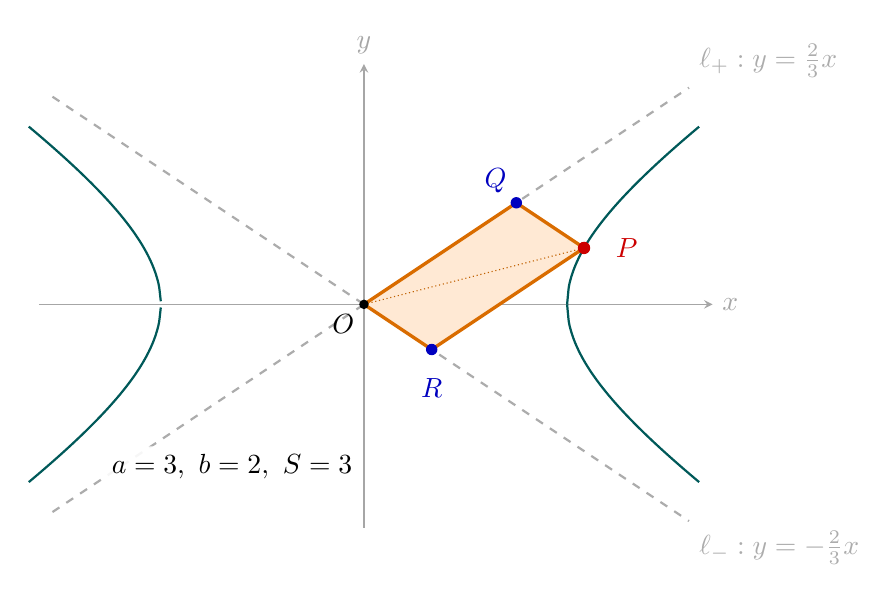
\begin{tikzpicture}[scale=0.86,>=stealth]
  \draw[->,gray!70] (-4.8,0)--(5.15,0) node[right] {$x$};
  \draw[->,gray!70] (0,-3.3)--(0,3.55) node[above] {$y$};
  \draw[gray!65,dashed,thick] (-4.6,-3.06667)--(4.8,3.2)
    node[above right] {$\ell_+:y=\frac23x$};
  \draw[gray!65,dashed,thick] (-4.6,3.06667)--(4.8,-3.2)
    node[below right] {$\ell_-:y=-\frac23x$};
  \draw[teal!70!black,thick,samples=80,domain=3:4.95,smooth]
    plot (\x,{(2/3)*sqrt(\x*\x-9)});
  \draw[teal!70!black,thick,samples=80,domain=3:4.95,smooth]
    plot (\x,{-(2/3)*sqrt(\x*\x-9)});
  \draw[teal!70!black,thick,samples=80,domain=-4.95:-3,smooth]
    plot (\x,{(2/3)*sqrt(\x*\x-9)});
  \draw[teal!70!black,thick,samples=80,domain=-4.95:-3,smooth]
    plot (\x,{-(2/3)*sqrt(\x*\x-9)});
  \coordinate (O) at (0,0);
  \coordinate (Q) at (2.25,1.5);
  \coordinate (R) at (1,-0.6666666667);
  \coordinate (P) at (3.25,0.8333333333);
  \fill[orange!17] (O)--(Q)--(P)--(R)--cycle;
  \draw[orange!85!black,very thick] (O)--(Q)--(P)--(R)--cycle;
  \draw[orange!75!black,densely dotted] (O)--(P);
  \fill (O) circle(2pt) node[below left] {$O$};
  \fill[blue!75!black] (Q) circle(2.4pt) node[above left] {$Q$};
  \fill[blue!75!black] (R) circle(2.4pt) node[below=7pt] {$R$};
  \fill[red!80!black] (P) circle(2.6pt) node[right=8pt] {$P$};
  \node[fill=white,fill opacity=.9,text opacity=1,rounded corners=2pt,
    inner sep=3pt] at (-1.95,-2.4) {$a=3,\ b=2,\ S=3$};
\end{tikzpicture}
